
\section{Nonlinear Theory}
\sectionframe{3}{Nonlinear Theory}


%--------------------------
\myframe{Linear vs Nonlinear Kalman Filtering}{%
    \begin{itemize}
        \item \textbf{Linear Kalman Filter (KF)}: Assumes linear system dynamics and measurement models.

        \pause
        \medskip
        \item \textbf{Nonlinear versions}:
        \begin{itemize}
            \item \textbf{Extended Kalman Filter (EKF)}: Linearizes nonlinear models using Taylor series expansion.
            \item \textbf{Unscented Kalman Filter (UKF)}: Uses deterministic sampling to capture mean and covariance of nonlinear transformations.
            \item \textbf{Other variants}: E.g. Particle Filters (PFs), use random sampling to approximate any underlying distribution.
        \end{itemize}
    \end{itemize}

    \pause
    \medskip
    \centering
    \begin{tabular}{l|lp{2cm}p{4cm}}
        \textbf{Estimator} & \textbf{Model} & \textbf{Assumed Distribution} & \textbf{Computational Cost}\\
        \hline
        \hline
        KF & Linear  & Gaussian  & Low \\
        \hline
        EKF & Locally Linear  & Gaussian  & Low/Medium (depends on Jacobians) \\
        \hline
        UKF & Nonlinear  & Gaussian  & Medium \\
        \hline
        PFs & Nonlinear  & Arbitrary  &  High 
    \end{tabular}

}


%-------------------------------------------------------------------------------
\subsection{Extended Kalman Filter}

%--------------------------
\myframe{Extended Kalman Filter (EKF): essentials and notation}{%
    \begin{itemize}
        \item Linearizes nonlinear functions $f(x,u)$ and $h(x)$ around current estimate.
        \item Same equations as linear KF, but with linearized matrices.
        \item Limitations: Linearization errors, Jacobian computation.
    \end{itemize}

    \pause
    \medskip
    Consider a discrete-time\footnote{Here we make use of $k$ or $t_k$ to denote
    discrete-time instants since $t$ will later be used to denote continuous
    time.} non-linear state model of the form

    \begin{align*}
        \x(k+1) &= f(\x(k), \u(k)) + \v(k),\quad \v\sim\N(0,Q)\\
        \y(k)   &= h(\x(k)) + \w(k),\quad \w\sim\N(0,R)
    \end{align*}

    under the usual assumptions $\v\perp\w\perp\xzero$,
    \pause
    and denote the Jacobian matrices

    $$
        F_k = \left.\frac{\partial f}{\partial x}\right|_{\hat{x}_{k|k}}\qquad
        H_k = \left.\frac{\partial h}{\partial x}\right|_{\hat{x}_{k+1|k}}
    $$
}


%--------------------------
\myframe{EKF: discrete-time equations}{%

\begin{enumerate}
    \item Prior estimates
        \begin{itemize}
            \item State: $\xhat(k+1|k) = f(\xhat(k|k), \u(k))$
            \item Variance: $P(k+1|k) = F_kP(k|k)F_k^T + Q$,
        \end{itemize}

    \pause
    \medskip
    \item Measurement update
        \begin{itemize}
            \item State: $\xhat(k+1|k+1) = \xhat(k+1|k) + L(k+1)\left[\y(k+1)-h\left(\xhat(k+1|k)\right)\right]$
            \item Variance: $P(k+1|k+1) = (I - L(k+1) H_k) P(k+1|k)$ 

            \medskip
            \item $L(k+1) = P(k+1|k) H_k^T \Lambda(k+1)^{-1}$
            \item $\Lambda(k+1) = H_kP(k+1|k)H_k^T + R$ 
        \end{itemize}

    \pause
    \medskip
    \item Initial conditions
        \begin{itemize}
            \item $\xhat(0|-1)=\E[\x(t_0)]$
            \item $P(0|-1)=\Var[\x(t_0)]$  
        \end{itemize}
\end{enumerate}

\pause
\medskip
Nonlinearity used to properly propagate the prior estimate and the measurement
model to compute the pseudo innovation.

}

%--------------------------
\myframe{EKF: generalization - continuous-discrete equations}{%

    The EKF is also used in more general setups of continuous-discrete systems.

    \pause
    \medskip
    Consider a continuous-time state-model with sampled
    measurements at discrete instants $t_k$ (possibly non uniform)
    %
    \begin{align*}
        \dot{\x}(t) &= f(\x(t)) + \xi(t)\\
        \y(t_k) &= h(\x(t_k)) + \w(t_k) 
    \end{align*}
    %
    being $\xi$ white noise of intensity $Q\geq0$; $\w(t_k)$ white of variance
    $R>0$ and $\{\xi(t)\}\perp\{\w(t_k)\}\perp\x(t_0)$. $f,h\in\C^1$.
    %

    \pause
    Let $\Phi(t,s,\overline{\x})$ be the fundamental matrix\footnote{Matrix
    satisfying the Volterra equation which, for constant F, equals
    $\Phi(t,s)=e^{F(t-s)}$.} associated to the time-varying linear system
    $\dot{\z}=F(\overline{\x}(t))\z$ where $F(\overline{\x}(t))= \frac{\partial
    f}{\partial x}|_{\x=\overline{\x}(t)}$ and define
    $$
        Q(t_k) := \int_{t_k}^{t_{k+1}} \Phi(t_{k+1},s,\overline{\x})Q\Phi(t_{k+1,s},\overline{\x})^T ds
    $$

    Under these conditions, the equations generalize as follows.

}

%--------------------------
\myframe{EKF: generalization - continuous-discrete equations}{%
    
    \begin{enumerate}
        \setcounter{enumi}{0}
        \item Prior estimates
    \end{enumerate}
    \begin{itemize}
        \item State:
            \begin{itemize}
                \item Resolve $\dot{\overline{\x}}(t)=f(\overline{\x}(t))$, $t\in[t_k,t_{k+1}]$, $\overline{\x}(t_k)=\xhat(k|k)$ 
                \item Set $\xhat(k+1|k)=\overline{\x}(t_{k+1})$
            \end{itemize}
        \item Variance: 
            \begin{itemize}
                \item $P(k+1|k) = \Phi(k|k)P(k|k)\Phi(k|k)^T + Q(k)$, $\Phi(k|k):=\Phi(k+1,k,\xhat(k|k))$
                \item Alternative CT Riccati: $\dot{P}(t) = F(t)P(t) + P(t)F(t)^T + Q(t)$
            \end{itemize}
    \end{itemize}

    \pause
    \begin{enumerate}
        \setcounter{enumi}{1}
        \item Measurement update
    \end{enumerate}
    \begin{itemize}
        \item State:
            \begin{itemize}
                \item $\xhat(k+1|k+1) = \xhat(k+1|k) + L(k+1)\left[\y(k+1)-h\left(\xhat(k+1|k)\right)\right]$
                \item $L(k+1) = P(k+1|k) H(k+1|k)^T \Lambda(k+1)^{-1}$
                \item $\Lambda(k+1) = H(k+1|k)P(k+1|k)H(k+1|k)^T + R$ 
                \item $H(k+1|k) := H(\xhat(k+1|k)) = \frac{\partial h}{\partial x}|_{\x=\xhat(k+1|k)}$
            \end{itemize}
        \item Variance: $P(k+1|k+1) = (I - L(k+1) H(k+1|k)) P(k+1|k)$ 
    \end{itemize}

    with initial conditions $\xhat(0,-1)=\E[\x(t_0)], P(0|-1)=\Var[\x(t_0)]$

}


%--------------------------
\myframe{EKF: observations}{%

\begin{itemize}
    \item The linearized model is used only to compute $L(k)$.
    
    \pause
    \item The statistical interpretation of $\xhat(k+1|k)$ and $\xhat(k|k)$ can
    not in general be drawn being both non-linear functions of the data.

    \pause
    \item The algorithm is much more computationally intense. It requires
    computation of $H$ and $\Phi$ at every step, hence $L$ cannot be precomputed
    offline.
    
    \pause
    \item Adding a linear additive term $B\u(t)$ for an input component does not
    essentially complicate the filter equations.
\end{itemize}

\pause
To avoid explicit integration, when the signals
are sufficiently slow w.r.t. the sampling time, a full DT
scheme is used, by discretizing the CT dynamics, e.g.,
%
$$
\x(k+1) = \hat{f}_k(\x(k)) \overset{Euler}{=} \x(k) + (t_{k+1}-t_k)f(\x(k))
$$
also used to propagate the prior estimated state in the filter equations
%
$$
\xhat(k+1|k) = \hat{f}_k(\xhat(k|k))
$$

All other equations remain the same assuming now $\Phi(k|k)=\frac{\partial \hat{f}_k}{\partial x}|_{\x=\xhat(k|k)}$.

}


%-------------------------------------------------------------------------------
\subsection{Unscented Kalman Filter}

%--------------------------
\myframe{Unscented Kalman Filter (UKF)}{%
    \begin{itemize}
        \item Uses sigma points to capture higher-order moments: for any random
        vector $\x$, sigma points are a set of any $N$ vectors satisfying:
        \begin{itemize}
            \item first order: weighted average of points corresponds to $\E[\x]$
            \item second order: weighted average of points covariance corresponds to $\Var[\x]$ 
        \end{itemize}
        The critical point is to find the right choice of weights: for this
        standard approaches exists.

        \pause
        \item UKF usually generates $2n+1$ sigma points where $n$ is state dimension.

        \pause
        \item Propagates sigma points through nonlinear functions.
        
        \pause
        \item Reconstructs mean and covariance from transformed sigma points.
        
        \pause
        \item \textit{Main Advantages}:
        \begin{itemize}
            \item No Jacobian required wrt EKF
            \item  better handling of nonlinearities since $P$ is estimated
            considering nonlinear transforms.
        \end{itemize}
    \end{itemize}

\pause
\medskip
\textit{UKF equations are not difficult but heavy in notation. We'll see them in
code rather than on slides.}

}

%--------------------------
\myframe{UKF: graphical representation}{

\centering
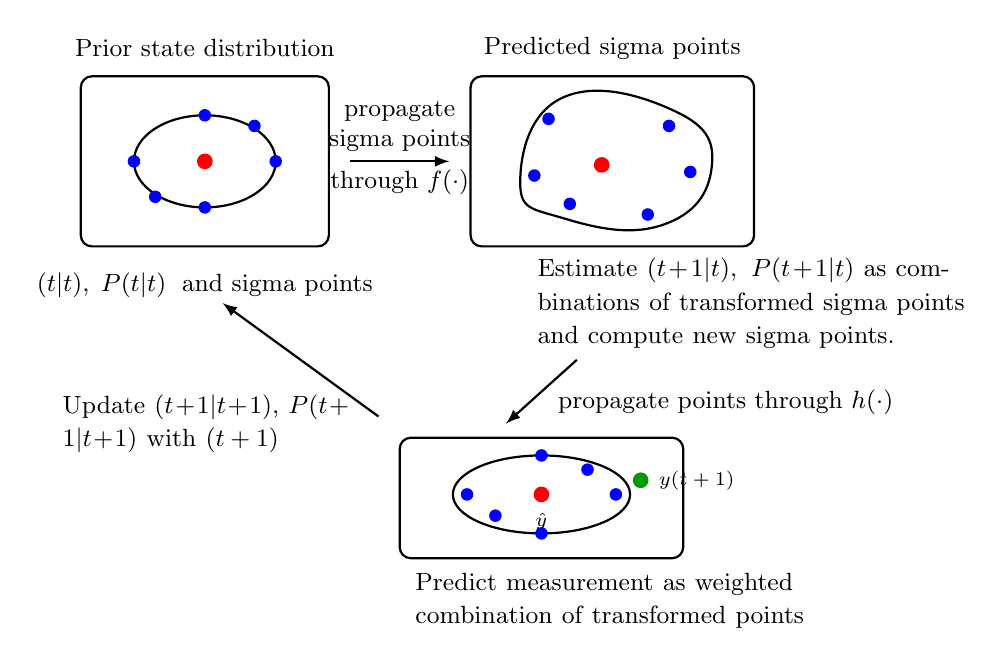
\begin{tikzpicture}[scale=0.9, >=latex]

    % Styles
    \tikzstyle{statecloud}=[draw, rounded corners, thick]
    \tikzstyle{arrow}=[->, thick]
    \tikzstyle{sigmapt}=[circle, fill=blue, inner sep=1.6pt]
    \tikzstyle{meanpt}=[circle, fill=red, inner sep=2pt]

    %-------------------------
    % Prior state box
    %-------------------------
    \draw[statecloud] (0,0.3) rectangle (3.5,2.7);
    \node at (1.75,3.1) {\small Prior state distribution};
    \node at (1.75,-0.25) {\small $\xhat(t|t),\;P(t|t)$\; and sigma points};

    % Prior ellipse
    \draw[thick] (1.75,1.5) ellipse (1.0 and 0.65);

    % Prior sigma points
    % \node[meanpt,label=below:{\scriptsize $\hat x$}] at (1.75,1.5) {};
    \node[meanpt] at (1.75,1.5) {};
    \node[sigmapt] at (2.75,1.5) {};
    \node[sigmapt] at (0.75,1.5) {};
    \node[sigmapt] at (1.75,2.15) {};
    \node[sigmapt] at (1.75,0.85) {};
    \node[sigmapt] at (2.45,2.0) {};
    \node[sigmapt] at (1.05,1.0) {};

    %-------------------------
    % Propagation arrow
    %-------------------------
    \draw[arrow] (3.8,1.5) -- (5.2,1.5);
    \node at (4.5,2.2) {\small propagate};
    \node at (4.5,1.8) {\small sigma points};
    \node at (4.5,1.2) {\small through $f(\cdot)$};

    %-------------------------
    % Predicted state box
    %-------------------------
    \draw[statecloud] (5.5,0.3) rectangle (9.5,2.7);
    \node at (7.5,3.1) {\small Predicted sigma points};
    \node[text width=5.5cm] at (9.5,-0.5) {%
        \small Estimate $\xhat(t\!+\!1|t),\;P(t\!+\!1|t)$ as
        combinations of transformed sigma points and
        compute new sigma points.
        };

    % Nonlinear transformed cloud
    \draw[thick] plot[smooth cycle, tension=0.8] coordinates {
        (6.2,1.2) (6.8,2.4) (8.4,2.2) (8.9,1.4) (8.2,0.6) (6.8,0.7)
    };

    % Predicted sigma points
    % \node[meanpt,label=below:{\scriptsize $\hat x^-$}] at (7.35,1.45) {};
    \node[meanpt] at (7.35,1.45) {};
    \node[sigmapt] at (6.6,2.1) {};
    \node[sigmapt] at (8.3,2.0) {};
    \node[sigmapt] at (8.6,1.35) {};
    \node[sigmapt] at (8.0,0.75) {};
    \node[sigmapt] at (6.9,0.9) {};
    \node[sigmapt] at (6.4,1.3) {};

    %-------------------------
    % Measurement projection arrow
    %-------------------------
    \draw[arrow] (7,-1.3) -- (6,-2.2);
    \node at (9.1,-1.9) {\small propagate points through $h(\cdot)$};

    %-------------------------
    % Measurement box
    %-------------------------
    \draw[statecloud] (4.5,-4.1) rectangle (8.5,-2.4);
    % \node at (7.5,-1.95) {\small Predicted measurement};
    \node[text width=5cm] at (7.5,-4.7) {\small Predict measurement as weighted combination of transformed points};
    % \node at (7.5,-5.3) {\small $\hat y(t\!+\!1),\;S(t\!+\!1)$};

    % Measurement ellipse
    \draw[thick] (6.5,-3.2) ellipse (1.25 and 0.55);

    % Measurement sigma points
    \node[meanpt,label=below:{\scriptsize $\hat y$}] at (6.5,-3.2) {};
    \node[sigmapt] at (7.55,-3.2) {};
    \node[sigmapt] at (5.45,-3.2) {};
    \node[sigmapt] at (6.5,-2.65) {};
    \node[sigmapt] at (6.5,-3.75) {};
    \node[sigmapt] at (7.15,-2.85) {};
    \node[sigmapt] at (5.85,-3.5) {};

    % Actual measurement
    \node[circle, fill=green!60!black, inner sep=2pt,
          label=right:{\scriptsize $y(t+1)$}] at (7.9,-3) {};

    %-------------------------
    % Update arrow back
    %-------------------------
    % \draw[arrow] (9.9,-1.0) .. controls (11.0,-1.0) and (11.0,2.2) .. (9.7,2.2);
    \draw[arrow] (4.2,-2.1) -- (2,-0.5);

    % Posterior label inside predicted box
    \node[text width=3.7cm] at (1.8,-2.2) {\small Update $\xhat(t\!+\!1|t\!+\!1)$, $P(t\!+\!1|t\!+\!1)$ with $\y(t+1)$};

\end{tikzpicture}

}

%-------------------------------------------------------------------------------
\subsection{Particle Filters}

%--------------------------
\myframe{Particle Filters (PFs)}{

Particle Filters are a family rather than a single estimation algorithm.

\medskip
General idea:
\begin{itemize}
    \item use many samples/particle
    \item use random sampling to approximate any underlying distribution
    \item often exploit a \textit{genetic} approach consisting of a
    selection/updating step alternate with a mutation/prediction step
\end{itemize}

\medskip
Common implementations are:
\begin{itemize}
    \item Markov Chain Monte Carlo
    \item Sequential Importance Sampling (SIS)
    \item Sequential Importance Resampling (SIR)
\end{itemize}

}